% (c) 2012-2013 Claudio Carboncini - claudio.carboncini@gmail.com
% (c) 2012-2014 Dimitrios Vrettos - d.vrettos@gmail.com
% (c) 2014 Daniele Masini - d.masini.it@gmail.com

\chapter{Approfondimenti su relazioni e insiemi}

\section{Particolari relazioni d'equivalenza}

\subsection{La costruzione dell'insieme dei numeri interi relativi}\label{sect:ins_numeri_interi_relativi}

\epigraph{Dio fece i numeri naturali, tutto il resto è opera dell'uomo.}{\scshape{L. Kronecker}}

\begin{exrig}
 \begin{esempio}
 \label{ex:E.1}
Nell'insieme
\[A = \{(4;5)\text{, }(7;8)\text{, }(0;1)\text{, }(2;3)\text{, }(5;4)\text{, }(12;13)\text{, }(10;9)\text{, }(5;5)\text{, }(1;0)\text{, }(4;4)\text{, }(0;0)\}\]
sottoinsieme del prodotto cartesiano~$\insN \times \insN$, considera la relazione $\Rel$ così definita:
``$(m;n)$ è in relazione con $(p;q)$ se e solo se la somma di~$m$ con~$q$ è uguale alla somma di~$n$ con~$p$''.
In linguaggio matematico:~$(m;n) \,\Rel\, (p;q) \Leftrightarrow m+q = n+p$.

\begin{itemize*}
\item Completa il suo grafo~(figura~\ref{fig:E.1}) e deduci le proprietà;
\item costruisci e rappresenta con diagrammi di Eulero-Venn l'insieme quoziente~$A/\Rel$;
\item quante classi d'equivalenza hai ottenuto?
\item è vero che ciascuna di esse può essere rappresentata da una coppia avente almeno un elemento nullo?
\item scrivi i rappresentanti delle classi d'equivalenza.
\end{itemize*}
 \end{esempio}
\end{exrig}

 \begin{figure}[hb]
  \centering% (c) 2012 Dimitrios Vrettos - d.vrettos@gmail.com
\begin{tikzpicture}[x=10mm, y=10mm]

  \node[ellipse, minimum height=4cm,, minimum width=6cm, draw] (A) at (0,0) {};

  \begin{scope}[fill=CornflowerBlue]
    \filldraw (-2,.3) circle (2pt) node (a) {};
    \node[left] at (-2,.3) {$(7;8)$};
    
    \filldraw (.5,.5) circle (2pt) node (b) {};
    \node[below] at (.5,.5) {$(2;3)$};
    
    \filldraw (-.4,1.4) circle (2pt) node (c) {};
    \node[above] at (-.4,1.4)  {$(0;1)$};

    \filldraw (-1,-.3) circle (2pt) node (d) {};
    \node[above] at (-1,-.3)  {$(4;4)$};

    \filldraw (1,-.6) circle (2pt) node (e) {};
    \node[below] at (1,-.6)  {$(0;0)$};

    \filldraw (2.1,-.3) circle (2pt) node (f) {};
    \node[above] at (2.1,-.3)  {$(5;5)$};

    \filldraw (-2,-.5) circle (2pt) node (g) {};
    \node[below] at (-2,-.5)  {$(5;4)$};

    \filldraw (-.1,-.8) circle (2pt) node (h) {};
    \node[below] at (-.1,-.8)  {$(1;0)$};

    \filldraw (1.4,.7) circle (2pt) node (i) {};
    \node[right] at (1.4,.7)  {$(12;13)$};

    \filldraw (-1.2,1.4) circle (2pt) node (j) {};
    \node[below] at (-1.2,1.4)  {$(4;5)$};

    \filldraw (-.4,-1.5) circle (2pt) node (k) {};
    \node[left] at (-.4,-1.5)  {$(10;9)$};
  \end{scope}

  \begin{scope}[-,smooth,thick]
    \draw[Maroon] (a) .. controls +(30:1cm) and +(150:.5cm) .. (b);
    \draw[purple] (b) .. controls +(30:.5cm) and +(0:0.5cm) .. (c);
    \draw[orange] (d) .. controls +(0:1cm) and +(180:1cm) .. (e);
    \draw[OliveGreen] (e) .. controls +(0:1cm) and +(-90:.5cm) .. (f);
    \draw[RedOrange] (g) .. controls +(0:1cm) and +(180:.5cm) .. (h);
  \end{scope}
\end{tikzpicture}

 \caption{Esempio~\ref{ex:E.1}.}\label{fig:E.1}
 \end{figure}

Proviamo ora a generalizzare quanto ottenuto.
Consideriamo la relazione~$\Rel$ definita nell'esempio precedente su tutto il dominio~$\insN\times\insN$; essendo~$\insN\times\insN$
costituito da infiniti elementi non possiamo rappresentare il grafo della relazione, ma possiamo comunque studiarne le proprietà per
stabilire se anche in questo insieme si mantengono le conclusioni raggiunte nell'esempio.

\paragraph{La relazione è riflessiva} per qualunque coppia~$(m;n)$ di~$\insN\times\insN$ si ha~$(m;n) \,\Rel\, (m;n)$.

Infatti applicando il predicato della relazione si ottiene l'uguaglianza~$m+n = n+m$, vera qualunque siano i numeri naturali
$m$ ed~$n$ poiché l'addizione in~$\insN$ gode della proprietà commutativa. Con riferimento all'attività precedente hai potuto infatti
mettere il cappio sopra ogni coppia: ad esempio è vero che~$(4;5) \,\Rel\, (4;5)$ poiché $4+5 = 5+4$.

\paragraph{La relazione è simmetrica} per qualunque coppia~$(m;n)$ e~$(p;q)$ appartenenti a~$\insN\times\insN$, se~$(m;n)\,\Rel\,(p;q)$ allora~$(p;q)\,\Rel\, (m;n)$.

Infatti se~$(m;n)\,\Rel\,(p;q)$ si ha~$m+q = n+p$; per la proprietà commutativa dell'addizione in~$\insN$ si ha anche~$p+n=q+m$,
uguaglianza che assicura la validità della relazione $\Rel$ tra la coppia~$(p;q)$ e~$(m;n)$.

Nell'esercizio precedente, ad esempio, la coppia~$(5;4)$ è in relazione con la coppia~$(10;9)$ perché è vero che~$5+9 = 4+10$;
da questa è anche vero che~$10+4 = 9+5$,
uguaglianza che assicura~$(10;9)\,\Rel\,(5;4)$: nel grafo hai usato archi per evidenziare coppie in relazione.

\paragraph{La relazione è transitiva} se~$(m;n)\,\Rel\,(p;q)$ e~$(p;q)\,\Rel\,(s;t)$ allora~$(m;n)\,\Rel\,(s;t)$,
per qualunque terna di coppie~$(m;n)$, $(p;q)$, $(s;t)$ appartenenti a~$\insN\times\insN$.

Infatti se~$(m;n)\,\Rel\,(p;q)$ e~$(p;q)\,\Rel\,(s;t)$ si ha~$m+q = n+p$ e~$p+t = q+s$; sommando membro a membro le precedenti
uguaglianze si ottiene
\begin{align*}
 m+q + p+t &= n+p + q+s\\
 \Rightarrow\: (m+t)+(q+p) &= (n+s)+(q+p)
\end{align*}
per le proprietà commutativa e associativa dell'addizione in~$\insN$. Confrontando i membri dell'uguaglianza si deduce che~$m+t = n+s$,
e quest'ultima assicura la verità dell'affermazione~$(m;n)\,\Rel\,(s;t)$.

Riferendoti all'esempio svolto sopra hai potuto stabilire che~$(5;4)\,\Rel\,(10;9)$ e~$(10;9)\,\Rel \,(1;0)$
poiché $5+9=4+10$ e~$10+0=9+1$. Procediamo come nel ragionamento precedente e sommiamo membro a membro le due uguaglianze
\begin{align*}
 5+9+10+0 &= 4+10+9+1\\
\Rightarrow\: (5+0)+(9+10) &= (4+1)+(10+9)\\
\Rightarrow\: 5+0 &= 4+1\text{,}
\end{align*}
che assicura la verità di~$(5;4)\,\Rel\,(1;0)$.% Nella figura~\ref{fig:E.2} della relazione compaiono ellissi aventi come sfonfo grigio coppie in relazione.

\begin{figure}[t]
 \centering% (c) 2012 Dimitrios Vrettos - d.vrettos@gmail.com
\begin{tikzpicture}[x=10mm, y=10mm]

  \node[ellipse, minimum height=6cm, minimum width=8cm, draw] (A) at (0,0) {};
  \node[above] at (0,3) {$(\insN\times\insN)/\Rel$};
  
  \node[ellipse, minimum height=1.5cm, minimum width=1.5cm, draw] (B) at (-2.8,1) {};

  \node[ellipse, minimum height=1.5cm, minimum width=2.1cm, draw] (C) at (-.8,1.4) {};

  \node[ellipse, minimum height=1.8cm, minimum width=2.3cm, draw] (D) at (-1.5,-.4) {};

  \node[ellipse, minimum height=1.8cm, minimum width=2.3cm, draw] (E) at (1.5,1.1) {};

  \node[ellipse, minimum height=1cm, minimum width=1cm, draw] (F) at (3,-.8) {};

  \node[ellipse, minimum height=1.6cm, minimum width=1.3cm, draw] (G) at (1,-1.2) {};

  \node[ellipse, minimum height=1cm, minimum width=2cm, draw] (F) at (-.8,-2) {};

  \begin{scope}[fill=CornflowerBlue]
    \filldraw (-2.8,1) circle (2pt) node (a) {};
    \node[above] at (-2.8,1) {$(31;17)$};

    \filldraw (-.4,1.4) circle (2pt) node (c) {};
    \node[above] at (-.4,1.4)  {$(0;0)$};

    \filldraw (-1.2,1.4) circle (2pt) node (j) {};
    \node[below] at (-1.2,1.4)  {$(3;3)$};

    \filldraw (-1,-.3) circle (2pt) node (d) {};
    \node[above] at (-1,-.3)  {$(1;3)$};

    \filldraw (-2,-.5) circle (2pt) node (g) {};
    \node[below] at (-2,-.5)  {$(0;2)$};

    \filldraw (1.5,1.5) circle (2pt) node (b) {};
    \node[below] at (1.5,1.5) {$(1;0)$};

    \filldraw (1.4,.7) circle (2pt) node (i) {};
    \node[right] at (1.4,.7)  {$(5;4)$};

    \filldraw (3,-1) circle (2pt) node (f) {};
    \node[above] at (3,-1)  {$(6;9)$};

    \filldraw (1,-1.3) circle (2pt) node (h) {};
    \node[below] at (1,-1.3)  {$(3;7)$};

    \filldraw (1,-.6) circle (2pt) node (e) {};
    \node[below] at (1,-.6)  {$(0;4)$};

    \filldraw (-.4,-2) circle (2pt) node (k) {};
    \node[left] at (-.4,-2)  {$(5;1)$};
  \end{scope}

\end{tikzpicture}

 \caption{Insieme quoziente~$(\insN\times\insN)/\Rel$ nel quale sono stati rappresentati solo alcuni elementi.}\label{fig:E.2}
\end{figure}

\conclusione La relazione~$\Rel$ così introdotta nell'insieme delle coppie ordinate di numeri naturali è una relazione d'equivalenza che determina
una partizione in classi d'equivalenza dell'insieme~$\insN\times\insN$, ovvero l'insieme quoziente $(\insN\times\insN)/\Rel$ (figura~\ref{fig:E.2}).

Analizzando con attenzione~$(\insN\times\insN)/\Rel$, possiamo determinare quale coppia ci conviene assumere come rappresentante di ciascuna classe
d'equivalenza. Si può osservare che:
\begin{itemize*}
\item coppie formate da elementi uguali appartengono alla stessa classe d'equivalenza che può quindi essere rappresentata dalla coppia~$(0;0)$;
\item la coppia~$(m;n)$ con~$m>n$ è equivalente alla coppia~$(m-n;0)$ essendo
\[m+0 = n+m-n;\]
pertanto, in tal caso, la classe d'equivalenza della coppia~$(m;n)$ può essere rappresentata dalla coppia~$(m-n;0)$;
\item la coppia~$(m;n)$ con~$m<n$ è equivalente alla coppia~$(0; n-m)$ essendo
\[m+n-m = n+0;\]
pertanto, in tal caso, la classe d'equivalenza della coppia~$(m;n)$ può essere rappresentata dalla coppia~$(0;n-m)$.
\end{itemize*}
Per esercizio, determina la coppia avente un elemento nullo ed equivalente a~$(31;17)\ldots\ldots$, $(6;9)\ldots\ldots$, $(5;1)\ldots\ldots$

\conclusione Ciascuna classe d'equivalenza può essere rappresentata da una coppia di numeri naturali avente almeno un elemento nullo.

L'insieme quoziente~$(\insN\times\insN)/\Rel$ può essere pertanto rappresentato dalle sue classi di equivalenza come nella figura~\ref{fig:E.3}.
\begin{figure}[t]
 \centering% (c) 2012 Dimitrios Vrettos - d.vrettos@gmail.com
\begin{tikzpicture}[x=10mm, y=10mm]

\node[ellipse, minimum height=6cm,, minimum width=8cm, draw] (A) at (0,0) {};
\node[above] at (0,3) {$(\insN\times\insN)/\Rel$};

\begin{scope}[fill=CornflowerBlue]
\filldraw (-2.8,1) circle (2pt) node (a) {};
\node[above] at (-2.8,1) {$[(0;1)]$};

\filldraw (-.4,1.4) circle (2pt) node (c) {};
\node[above] at (-.4,1.4)  {$[(0;2)]$};

\filldraw (-1.2,1.4) circle (2pt) node (j) {};

\filldraw (-1,-.3) circle (2pt) node (d) {};
\node[above] at (-1,-.3)  {$[(0;4)]$};

\filldraw (-2,-.5) circle (2pt) node (g) {};
\node[below] at (-2,-.5)  {$[(0;0)]$};

\filldraw (1.5,1.5) circle (2pt) node (b) {};
\node[below] at (1.5,1.5) {$[(14;0)]$};

\filldraw (1.4,.7) circle (2pt) node (i) {};

\filldraw (3,-1) circle (2pt) node (f) {};

\filldraw (1,-1.3) circle (2pt) node (h) {};

\filldraw (1,-.6) circle (2pt) node (e) {};
\node[below] at (1,-.6)  {$[(3;0)]$};

\filldraw (-.4,-2) circle (2pt) node (k) {};
\node[left] at (-.4,-2)  {$[(1;0)]$};
\end{scope}

\end{tikzpicture}

 \caption{Alcune classi di equivalenza di~$(\insN\times\insN)/\Rel$.}\label{fig:E.3}
\end{figure}

\begin{definizione}
 Si chiama \emph{numero intero relativo} ogni classe d'equivalenza ottenuta introducendo in~$\insN\times\insN$ la
 relazione~$(m;n)\,\Rel\, (p;q) \Leftrightarrow m+q=n+p$.
 \end{definizione}

\begin{definizione}
Si chiama \emph{forma canonica} del numero intero relativo la coppia scelta come rappresentante della classe d'equivalenza.
\end{definizione}

Possiamo ad esempio dire che la classe di equivalenza~$[(3;7)]$ è un numero intero relativo e la sua forma canonica è~$(0;4)$.

\begin{definizione}
Si chiama \emph{numero intero positivo} la classe d'equivalenza~$[(n;0)]$ e si indica con il simbolo~$+n$.
\end{definizione}

\begin{definizione}
 Si chiama \emph{numero intero negativo} la classe d'equivalenza~$[(0;n)]$ e si indica con il simbolo~$-n$.
\end{definizione}

\begin{definizione}
 Si chiama \emph{zero} la classe d'equivalenza~$[(0;0)]$ e si indica con~$0$.
\end{definizione}

\begin{definizione}
 Si chiama \emph{valore assoluto del numero intero relativo} il numero naturale diverso da zero che compare nella sua forma canonica.
\end{definizione}

\begin{definizione}
 L'insieme~$(\insN\times \insN)/\Rel$ è chiamato \emph{insieme dei numeri interi relativi} e indicato con il simbolo~$\insZ$.
\end{definizione}

\osservazione L'insieme dei numeri interi relativi viene semplicemente chiamato insieme dei numeri interi.

Esso contiene tre sottoinsiemi~$\insZ^{+} =\{x \mid  x \text{ è intero positivo}\}$, $\insZ^{-} =\{x \mid  x \text{ è intero negativo}\}$
e l'insieme il cui unico elemento è lo zero~$\{0\}$. Scriviamo quindi~$\insZ = \insZ^{+}\cup \insZ^{-}\cup\{0\}$ e rappresentiamo con diagramma di Eulero-Venn di figura~\ref{fig:E.4}.

\begin{figure}[hbt]
 \centering% (c) 2012 Dimitrios Vrettos - d.vrettos@gmail.com
\begin{tikzpicture}[x=10mm, y=10mm]

\node[ellipse, minimum height=3cm,minimum width=8cm, draw] (A) at (0,0) {};
  \node[above] at (0,1.5) {$\insZ$};
  
%   \node[ellipse, minimum height=1cm, minimum width=1.5cm, draw] (B) at (-2.8,0) {};
  \node[above] at (-2.8,.4) {$\{0\}$};
  
%   \node[ellipse, minimum height=1.5cm, minimum width=2.1cm, draw] (C) at (-.8,.4) {};
  \node[below] at (-.8,-.35) {$\insZ^+$};
  
%   \node[ellipse, minimum height=1.8cm, minimum width=3cm, draw] (E) at (2,.1) {};
  \node[below left] at (2,-.7) {$\insZ^-$};

\draw (-2,1.3) -- (-2,-1.3);
\draw (1,1.46) -- (1,-1.46);
  \begin{scope}[fill=CornflowerBlue]
    \filldraw (-2.8,0) circle (2pt) node (a) {};
    \node[above] at (-2.8,0) {$0$};

    \filldraw (-.4,.4) circle (2pt) node (c) {};
    \node[above] at (-.4,.4)  {$+3$};

    \filldraw (-1.2,.4) circle (2pt) node (j) {};
    \node[below] at (-1.2,.4)  {$+34$};

    \filldraw (1.5,.5) circle (2pt) node (b) {};
    \node[below] at (1.5,.5) {$-124$};

    \filldraw (1.4,-.3) circle (2pt) node (i) {};
    \node[right] at (1.4,-.3)  {$-1$};

    \filldraw (2.5,0) circle (2pt) node (i) {};
    \node[right] at (2.5,0)  {$-8$};
  \end{scope}
\end{tikzpicture}
 \caption{Alcuni elementi dell'insieme dei numeri interi~$\insZ$.}\label{fig:E.4}
\end{figure}

Quando si debbano considerare solamente gli interi positivi e negativi si usa il simbolo~$\insZ_0$ col quale si indica che l'insieme dei numeri interi
relativi è stato privato dello zero:
\[\insZ_0 = \insZ^{+}\cup\insZ^{-} = \insZ -\{0\}.\]

\ovalbox{\risolvii \ref{ese:E.1}, \ref{ese:E.2}}

\subsection{La costruzione dell'insieme dei numeri razionali}\label{sect:ins_numeri_razionali}

Indichiamo con~$\insN_{0}$ l'insieme dei naturali privato dello zero, precisamente~$\insN_{0}=\insN-\{0\}$ e costruiamo l'insieme
$\insN\times\insN_{0}$; esso sarà costituito da tutte le coppie ordinate di numeri naturali di cui il secondo elemento è diverso da zero,
cioè~$(0;3)\in \insN\times\insN_{0}$ mentre~$(5;0)\notin\insN\times \insN_{0}$.
In questo insieme sia~$\Rel$ la relazione così definita~$(m;n)\,\Rel\, (p;q) \Leftrightarrow m\cdot q=n\cdot p$.

\begin{exrig}
 \begin{esempio}
\TabPositions{4cm}
Nella relazione definita sopra, indica se le seguenti frasi sono vere o false e dai la motivazione di quanto affermi.
\begin{itemize*}
\item $(3;5)\,\Rel\, (15;25)$ \tab\boxV\quad\boxF\qquad\dotfill;
\item $(3;9)\,\Rel\, (1;3)$ \tab\boxV\quad\boxF\qquad\dotfill;
\item $(8;9)\,\Rel\, (7;8)$ \tab\boxV\quad\boxF\qquad\dotfill;
\item $(0;6)\,\Rel\, (0;1)$ \tab\boxV\quad\boxF\qquad\dotfill
\end{itemize*}
 \end{esempio}
\end{exrig}

Analizziamo le proprietà della relazione appena definita:

\paragraph{La relazione è riflessiva} per qualunque~$(m;n)\in \insN\times\insN_{0}$ si ha~$(m;n)\,\Rel\, (m;n)$.

Infatti, applicando il predicato della relazione, si ottiene l'uguaglianza~$m\cdot n=n\cdot m$, vera qualunque siano i numeri naturali
$m$ ed~$n$ poiché la moltiplicazione in~$\insN$ gode della proprietà commutativa.

\paragraph{La relazione è simmetrica} per qualunque coppia~$(m;n)$ e~$(p;q)$ dell'insieme~$\insN\times\insN_{0}$ se $(m;n)\,\Rel\, (p;q)$ allora $(p;q)\,Rel\, (m;n)$.

Infatti, se~$(m;n)\,\Rel\,(p;q)$ si ha  $m\cdot q=n\cdot p$; per la proprietà commutativa della moltiplicazione in~$\insN$ si ha anche~$p\cdot n=q\cdot m$,
uguaglianza che assicura la validità della relazione tra la coppia~$(p;q)$ e~$(m;n)$.

\paragraph{La relazione è transitiva} se~$(m;n)\,\Rel\, (p;q)$ e~$(p;q)\,\Rel\, (s;t)$ allora~$(m;n)\,\Rel\,(s;t)$, per qualunque terna di coppie~$(m;n)$, $(p;q)$, $(s;t)$ appartenenti a~$\insN\times\insN_{0}$.

Infatti, se~$(m;n)\,\Rel\, (p;q)$ e~$(p;q)\,\Rel\, (s;t)$ sappiamo che  $m\cdot q=n\cdot p$ e che~$p\cdot t=q\cdot s$;
moltiplicando membro a membro le precedenti uguaglianze si ottiene
\begin{align*}
m\cdot q\cdot p\cdot t&=n\cdot p\cdot q\cdot s\\
\Rightarrow (m\cdot t)\cdot (q\cdot p)&=(n\cdot s)\cdot (q\cdot p)
\end{align*}
per le proprietà commutativa e associativa
della moltiplicazione in~$\insN$. Confrontando i membri dell'uguaglianza e dividendo per i fattori uguali si deduce che~$m\cdot t=n\cdot s$,
che assicura la verità dell'affermazione~$(m;n)\,\Rel\, (s;t)$.

\conclusione La relazione~$\Rel$ introdotta nell'insieme~$\insN\times \insN_{0}$ è una relazione d'equivalenza che determina
una partizione in classi d'equivalenza dell'insieme~$\insN\times \insN_{0}$, ovvero l'insieme quoziente $\insN\times \insN_{0}/\Rel$ (figura~\ref{fig:E.5}).

\begin{figure}[t]
 \centering% (c) 2012 Dimitrios Vrettos - d.vrettos@gmail.com
\begin{tikzpicture}[x=10mm, y=10mm]

  \node[ellipse, minimum height=6cm, minimum width=8cm, draw] (A) at (0,0) {};
  \node[above] at (0,3) {$(\insN\times\insN_0)/\Rel$};
  
  \node[ellipse, minimum height=1.5cm, minimum width=1.5cm, draw] (B) at (-2.8,1) {};

  \node[ellipse, minimum height=1.5cm, minimum width=2.1cm, draw] (C) at (-.8,1.4) {};

  \node[ellipse, minimum height=1.8cm, minimum width=2.3cm, draw] (D) at (-1.5,-.4) {};

  \node[ellipse, minimum height=1.8cm, minimum width=2.3cm, draw] (E) at (1.5,1.1) {};

  \node[ellipse, minimum height=1cm, minimum width=1cm, draw] (F) at (3,-.8) {};

  \node[ellipse, minimum height=1.6cm, minimum width=1.3cm, draw] (G) at (1,-1.2) {};

  \node[ellipse, minimum height=1cm, minimum width=2cm, draw] (F) at (-.8,-2) {};

  \begin{scope}[fill=CornflowerBlue]
    \filldraw (-2.8,1) circle (2pt) node (a) {};
    \node[above] at (-2.8,1) {$(31;17)$};

    \filldraw (-.4,1.4) circle (2pt) node (c) {};
    \node[above] at (-.4,1.4)  {$(9;9)$};

    \filldraw (-1.2,1.4) circle (2pt) node (j) {};
    \node[below] at (-1.2,1.4)  {$(3;3)$};

    \filldraw (-1,-.3) circle (2pt) node (d) {};
    \node[above] at (-1,-.3)  {$(0;4)$};

    \filldraw (-2,-.5) circle (2pt) node (g) {};
    \node[below] at (-2,-.5)  {$(0;2)$};

    \filldraw (1.5,1.5) circle (2pt) node (b) {};
    \node[below] at (1.5,1.5) {$(8;6)$};

    \filldraw (1.4,.7) circle (2pt) node (i) {};
    \node[right] at (1.4,.7)  {$(4;3)$};

    \filldraw (3,-1) circle (2pt) node (f) {};
    \node[above] at (3,-1)  {$(6;9)$};

    \filldraw (1,-1.3) circle (2pt) node (h) {};
    \node[below] at (1,-1.3)  {$(3;2)$};

    \filldraw (1,-.6) circle (2pt) node (e) {};
    \node[below] at (1,-.6)  {$(6;4)$};

    \filldraw (-.4,-2) circle (2pt) node (k) {};
    \node[left] at (-.4,-2)  {$(5;1)$};
  \end{scope}

\end{tikzpicture}
 \caption{Insieme quoziente~$\insN\times \insN_{0}/\Rel$ nel quale sono rappresentati alcuni elementi.}\label{fig:E.5}
\end{figure}

Vogliamo determinare la coppia da assumere come rappresentante di ciascuna classe d'equivalenza. Per fare questo associamo
a ciascuna coppia~$(a;b)$ di~$\insN\times\insN_{0}$ la frazione~$\dfrac{a}{b}$ e osserviamo che la relazione~$\Rel$ in~$\insN\times\insN_{0}$ prende significato
se trasferita nell'insieme delle frazioni dall'operazione che permette di costruire frazioni equivalenti.
\begin{exrig}
 \begin{esempio}
Presa la coppia~$(4;3)$ ad essa associamo la frazione~$\dfrac{4}{3}$; alla coppia~$(8;6)$ associamo la frazione~$\dfrac{8}{6}$.
Le coppie~$(4;3)$ e~$(8;6)$ stanno nella stessa classe d'equivalenza poiché $4\cdot 6=3\cdot 8$; le frazioni~$\dfrac{4}{3}$ e~$\dfrac{8}{6}$
sono equivalenti secondo l'usuale definizione.
 \end{esempio}
\end{exrig}

\conclusione Tutte le coppie appartenenti ad una classe d'equivalenza risultano associate ad una stessa frazione; scegliamo dunque come rappresentante
di ciascuna classe la frazione ridotta ai minimi termini, cioè nella quale numeratore e denominatore risultano primi tra loro.

L'insieme quoziente~$\insN\times\insN_{0}/\Rel$ può quindi essere rappresentato come nella figura~\ref{fig:E.6}.
\begin{figure}[t]
 \centering% (c) 2012 Dimitrios Vrettos - d.vrettos@gmail.com
\begin{tikzpicture}[x=10mm, y=10mm]

\node[ellipse, minimum height=5cm,, minimum width=7cm, draw] (A) at (0,0) {};
\node[above] at (0,2.5) {$\insN\times\insN_0/\Rel$};

\begin{scope}[fill=CornflowerBlue]
\filldraw (-2.8,1) circle (2pt) node (a) {};

\filldraw (-.4,1.4) circle (2pt) node (c) {};

\filldraw (-1.2,1.4) circle (2pt) node (j) {};
\node[below] at (-1.2,1.4)  {$[(\frac{2}{5})]$};

\filldraw (-1,-.3) circle (2pt) node (d) {};

\filldraw (-2,-.5) circle (2pt) node (g) {};
\node[below] at (-2,-.5)  {$[(0)]$};

\filldraw (1.5,1.5) circle (2pt) node (b) {};

\filldraw (1.4,.7) circle (2pt) node (i) {};
\node[below] at (1.4,.7)  {$[(\frac{4}{3})]$};

\filldraw (3,-1) circle (2pt) node (f) {};

\filldraw (1,-1.3) circle (2pt) node (h) {};

\filldraw (1,-.6) circle (2pt) node (e) {};
\node[below] at (1,-.6)  {$[(10)]$};

\filldraw (-.4,-2) circle (2pt) node (k) {};

\end{scope}
\end{tikzpicture}

 \caption{Alcune classi di equivalenza di~$\insN\times\insN_{0}/\Rel$.}\label{fig:E.6}
\end{figure}

\begin{definizione}
L'insieme quoziente~$\insN\times\insN_{0}/\Rel$ si chiama \emph{insieme dei numeri razionali assoluti} e si indica con il simbolo~$\insQ_{A}$.
\end{definizione}

\begin{definizione}
Si chiama \emph{numero razionale assoluto} ogni classe d'equivalenza ottenuta introducendo in~$\insN\times\insN_{0}$ la relazione~$\Rel$:
$(m;n)\,\Rel\, (p;q) \Leftrightarrow m\cdot q=n\cdot p$; esso viene rappresentato dalla frazione ad esso equivalente ridotta ai minimi termini.
\end{definizione}

Quanto abbiamo detto ci permette di passare dall'insieme delle frazioni ad un insieme di numeri che, benché scritti con il simbolo~$\dfrac{m}{n}$,
lo stesso usato per rappresentare una parte di una grandezza, hanno un significato completamente diverso dalla frazione.
D'altra parte, hai già visto nella secondaria di primo grado che al simbolo~$m/n$ si può attribuire il significato di quoziente della
divisione tra il numeratore e il denominatore e che i numeri razionali sono tutti quelli che si possono scrivere sotto forma di frazione.

\begin{exrig}
 \begin{esempio}
Completa la tabella e verifica se le coppie appartengono alla stessa classe di equivalenza, in questo caso indica il rappresentante della classe.
Le coppie rappresentano lo stesso numero razionale? In caso affermativo scrivi il simbolo del numero razionale.
\begin{center}
 \begin{tabular}{ccccc}
 \toprule
  Coppie & Stessa classe? & Rappr. classe & Stesso numero? & Simbolo numero\\
  $(1;2)$, $(3;2)$ & Sì &$\left[\frac{1}{2}\right]$ & Sì & $\frac{1}{2}$\\
  $(2;7)$, $(4;49)$ & & & & \\
  $(8;5)$, $(40;25)$ & & & & \\
  $(60;12)$, $(5;0)$ & & & & \\
  $(20;2)$, $(10;1)$ & & & & \\
  \bottomrule
 \end{tabular}
\end{center}
 \end{esempio}
\end{exrig}

\conclusione Se introduciamo la stessa relazione~$\Rel$ nell'insieme~$\insZ\times\insZ_{0}$, possiamo ottenere le seguenti definizioni.
\begin{definizione}
Si chiama \emph{insieme dei numeri razionali relativi} l'insieme quoziente~$(\insZ\times\insZ_{0})/\Rel$; esso si indica con il simbolo~$\insQ$.
\end{definizione}

\begin{definizione}
Si chiama \emph{numero razionale relativo} ogni classe d'equivalenza ottenuta introducendo in~$\insZ\times\insZ_{0}$ la relazione~$\Rel$:
$(m;n)\,\Rel\, (p;q) \Leftrightarrow m\cdot q=n\cdot p$; esso viene rappresentato da una frazione ridotta ai minimi termini dotata di segno.
\end{definizione}

\osservazione
L'insieme dei numeri razionali relativi viene semplicemente chiamato insieme dei numeri razionali.

L'insieme dei numeri razionali contiene tre sottoinsiemi~$\insQ^{+} =\{x \mid  x \text{ è razionale positivo}\}$, $\insQ^{-} =\{x \mid  x$ è razionale negativo$\}$
e l'insieme il cui unico elemento è lo zero~$\{0\}$. Scriviamo quindi~$\insQ = \insQ^{+}\cup \insQ^{-}\cup\{0\}$ e rappresentiamo con diagramma di Eulero-Venn nella figura~\ref{fig:E.7}.

\begin{figure}[htb]
 \centering% (c) 2012 Dimitrios Vrettos - d.vrettos@gmail.com
\begin{tikzpicture}[x=10mm, y=10mm]

  \node[ellipse, minimum height=3cm,minimum width=8cm, draw] (A) at (0,0) {};
  \node[above] at (0,1.5) {$\insQ$};
  \node[ellipse, minimum height=1cm, minimum width=1.5cm, draw] (B) at (-2.8,0) {};
  \node[above] at (-2.8,.4) {$\{0\}$};
  \node[ellipse, minimum height=1.5cm, minimum width=2.1cm, draw] (C) at (-.8,.4) {};
  \node[below] at (-.8,-.35) {$\insQ^+$};
  \node[ellipse, minimum height=1.8cm, minimum width=3cm, draw] (E) at (2,.1) {};
  \node[below left] at (2,-.7) {$\insQ^-$};

  \begin{scope}[fill=CornflowerBlue]
    \filldraw (-2.8,0) circle (2pt) node (a) {};
    \node[above] at (-2.8,0) {$0$};

    \filldraw (-.4,.4) circle (2pt) node (c) {};
    \node[above] at (-.4,.4)  {$+3$};

    \filldraw (-1.2,.4) circle (2pt) node (j) {};
    \node[below] at (-1.2,.4)  {$+\frac{3}{5}$};

    \filldraw (1.5,.5) circle (2pt) node (b) {};
    \node[right] at (1.5,.5)  {$-\frac{8}{3}$};

    \filldraw (1.4,-.3) circle (2pt) node (i) {};
    \node[right] at (1.4,-.3)  {$-1$};

    \filldraw (2.5,0) circle (2pt) node (i) {};
    \node[right] at (2.5,0)  {$-\frac{1}{2}$};
  \end{scope}
\end{tikzpicture}
 \caption{Alcuni elementi dell'insieme dei numeri razionali~$\insQ$.}\label{fig:E.7}
\end{figure}

Quando si debbano considerare solamente gli interi positivi e negativi si usa il simbolo~$\insQ_0$ col quale si indica che l'insieme dei numeri interi
relativi è stato privato dello zero, cioè
\[\insQ_0 = \insQ^{+}\cup\insQ^{-} = \insQ -\{0\}.\]

\ovalbox{\risolvii \ref{ese:E.3}, \ref{ese:E.4}, \ref{ese:E.5}}

\subsection{Classi di resti modulo n}

\begin{exrig}
 \begin{esempio}
Considera la relazione~$\Rel$: ``avere lo stesso resto nella divisione per~$3$'' introdotta nell'insieme
$A=\{n\in \insN \mid  0\le n\le 13\}$ e studiamone le proprietà.

Ricordiamo che il resto della divisione si calcola con l'operazione modulo indicata con $\bmod$; completiamo dunque le seguenti operazioni:
\begin{multicols}{4}
\noindent $0 \bmod~3=0$;\\ $1 \bmod~3=\ldots$;\\ $2 \bmod~3=\ldots$;\\$3 \bmod~3=\ldots$;\\$4 \bmod~3=\ldots$;\\$5 \bmod~3=\ldots$;\\$6 \bmod~3=0$;\\
$7 \bmod~3=\ldots$;\\$8 \bmod~3=\ldots$;\\$9 \bmod~3=\ldots$;\\$10 \bmod~3=\ldots$;\\$11 \bmod~3=2$;\\$12 \bmod~3=\ldots$;\\$13 \bmod~3=\ldots$
\end{multicols}
\begin{itemize*}
 \item La relazione~$\Rel$ è d'equivalenza; infatti \dotfill
\item completa l'insieme quoziente~$A/\Rel$;
\item quali sono i rappresentanti delle classi d'equivalenza?
\item sarebbe cambiato qualcosa se avessimo introdotto la stessa relazione nell'insieme $\insN$?
\item se sostituissimo~$\insN$ con~$\insZ$ cosa cambierebbe?
\end{itemize*}
 \end{esempio}

 \begin{esempio}
Nell'insieme~$\insN$ considera la relazione d'equivalenza~$\Rel$: ``avere lo stesso resto nella divisione per~$2$''.

Quante classi d'equivalenza puoi formare? Rappresenta l'insieme~$\insN/\Rel$. Quali sono i rappresentanti di ciascuna classe?
Riconosci in queste classi, particolari sottoinsiemi dell'insieme~$\insN$?
 \end{esempio}
\end{exrig}

Generalizziamo ora l'esercizio.
Fissato un numero naturale~$n>1$, considera la relazione~$\Rel$: ``avere lo stesso resto nella divisione intera per~$n$''
introdotta nell'insieme~$\insN$, studiane le proprietà e stabilisci se è d'equivalenza.
Osserviamo innanzitutto che nella divisione intera per~$n$ il resto si ottiene con l'operazione~$\bmod$ ed i possibili resti sono~0, 1, 2, \ldots, $n-1$,
cioè~$n$ valori.

\paragraph{La relazione è riflessiva} infatti per qualunque~$m\in \insN$ si ha~$m\,\Rel\, m$;
\paragraph{La relazione è simmetrica} infatti per qualunque~$p$ e~$q$ dell'insieme~$\insN$ se~$p\,\Rel\, q$ allora~$q\,\Rel\, p$.
Precisamente, se~$p\,\Rel\, q$ significa che~$p\bmod n=q\bmod n$ e per la proprietà simmetrica dell'uguaglianza possiamo scrivere
$q\bmod n=p\bmod n$, uguaglianza che assicura la validità della relazione tra~$q$ e~$p$;
\paragraph{La relazione è transitiva} se~$p\,\Rel\, q$ e~$q\,\Rel\, s$ allora~$p\,\Rel\, s$, per qualunque terna di naturali.
Infatti se~$p\,\Rel\, q$ significa~$p\bmod n=q\bmod n$ e se~$q\,\Rel\, s$ significa che~$q\bmod n=s\bmod n$;
per la proprietà transitiva dell'uguaglianza si ha~$p\bmod n=s\bmod n$, uguaglianza che assicura la validità della relazione tra~$p$ e~$s$.


\conclusione La relazione~$\Rel~$: ``avere lo stesso resto nella divisione intera per~$n$'', introdotta nell'insieme dei
numeri naturali, è una relazione d'equivalenza e permette quindi una partizione dell'insieme~$\insN$ in~$n$ classi d'equivalenza aventi
come rappresentanti tutti e soli i possibili resti della divisione intera per~$n$. L'insieme quoziente è formato da~$n$ elementi,
viene rappresentato come nella figura~\ref{fig:E.8} e viene chiamato \emph{insieme delle classi di resti modulo~$n$}.

\begin{figure}[b]
 \centering% (c) 2012 Dimitrios Vrettos - d.vrettos@gmail.com
\begin{tikzpicture}[x=10mm, y=10mm]

  \node[ellipse, minimum height=5cm,, minimum width=6cm, draw] (A) at (0,0) {};
  \node[above] at (0,2.5) {$\insN/\Rel$};
  \begin{scope}[fill=CornflowerBlue]
    \filldraw (-.4,1.4) circle (2pt) node (c) {};
    \node[above] at (-.4,1.4)  {$[0]$};

    \filldraw (-1.2,1.4) circle (2pt) node (j) {};

    \filldraw (-1,-.3) circle (2pt) node (d) {};
    \node[above] at (-1,-.3)  {$[2]$};

    \filldraw (-2,-.5) circle (2pt) node (g) {};
    \node[below] at (-2,-.5)  {$[n-1]$};

    \filldraw (1.5,1.5) circle (2pt) node (b) {};
    \node[below] at (1.5,1.5) {$[1]$};

    \filldraw (1.4,.7) circle (2pt) node (i) {};

    \filldraw (1,-.6) circle (2pt) node (e) {};
    \node[below] at (1,-.6)  {$[3]$};

    \filldraw (-.4,-2) circle (2pt) node (k) {};
    \node[left] at (-.4,-2)  {$[4]$};
  \end{scope}

\end{tikzpicture}

 \caption{Alcuni elementi dell'insieme delle classi di resti modulo~$n$.}\label{fig:E.8}
\end{figure}

L'insieme quoziente~$\insN/\Rel$ si indica anche col simbolo~$\insN_{n}$ dove l'indice~$n$ indica il numero rispetto al quale si è
eseguita l'operazione di modulo.

\ovalbox{\risolvii \ref{ese:E.6}, \ref{ese:E.7}, \ref{ese:E.8}, \ref{ese:E.9}}

\section{Insiemi finiti e insiemi infiniti}\label{sect:insiemi_finiti_e_infiniti}

Il concetto di ``corrispondenza biunivoca'' permette di affrontare il problema del confronto tra insiemi.
\begin{definizione}
 Due insiemi~$A$ e~$B$ si dicono \emph{equipotenti} se è possibile stabilire tra essi una corrispondenza biunivoca.
\end{definizione}

\begin{exrig}
 \begin{esempio}
Sia~$S$ l'insieme dei giorni della settimana e~$H$ l'insieme delle note musicali.
Sistemando gli elementi dei due insiemi come visualizzato nella seguente tabella ci rendiamo conto che tra di essi si può stabilire
una corrispondenza biunivoca, ottenuta semplicemente associando ad ogni giorno della settimana una e una sola nota musicale.
\begin{center}
 \begin{tabular}{cccccccc}
  \toprule
  $S$ & lunedì & martedì & mercoledì & giovedì & venerdì & sabato & domenica\\
    & $\downarrow$ & $\downarrow$ & $\downarrow$ & $\downarrow$ & $\downarrow$ & $\downarrow$ & $\downarrow$\\
  $H$ & do & re & mi & fa & sol & la & si\\
  \bottomrule
 \end{tabular}
\end{center}
Possiamo procedere anche scrivendo i giorni della settimana ciascuno su un foglietto da inserire in un'urna~$A_{1}$ e
facendo altrettanto con gli elementi dell'insieme~$H$ inseriti in un'urna~$A_{2}$; pescando alternativamente
un foglietto da~$A_{1}$ e uno da~$A_{2}$, ci accorgiamo che, esauriti i foglietti in~$A_{1}$ sono contemporaneamente
esauriti quelli in~$A_{2}$.

Concludiamo: l'insieme~$S$ è equipotente all'insieme~$H$.
Per esercizio mostra che l'insieme dei mesi dell'anno è equipotente all'insieme dei segni zodiacali.
 \end{esempio}
 
 \begin{esempio}
Consideriamo l'insieme~$\insN_{7}=\{x\in \insN\mid  0<x\le 7\}$ la cui rappresentazione per elencazione
è~$\insN_{7}=\{$1, 2, 3, 4, 5, 6, 7$\}$; come abbiamo fatto nell'esempio precedente, possiamo visualizzare la corrispondenza biunivoca
che si stabilisce tra~$S$, $H$ e~$\insN_{7}$ per mezzo della seguente tabella.
\begin{center}
 \begin{tabular}{cccccccc}
  \toprule
  $S$ & lunedì & martedì & mercoledì & giovedì & venerdì & sabato & domenica\\
    & $\downarrow$ & $\downarrow$ & $\downarrow$ & $\downarrow$ & $\downarrow$ & $\downarrow$ & $\downarrow$\\
  $H$ & do & re & mi & fa & sol & la & si\\
    & $\downarrow$ & $\downarrow$ & $\downarrow$ & $\downarrow$ & $\downarrow$ & $\downarrow$ & $\downarrow$\\
  $\insN_7$ & $1$ & $2$ & $3$ & $4$ & $5$ & $6$ & $7$\\
  \bottomrule
 \end{tabular}
\end{center}
Si verifica facilmente che il predicato ``essere equipotente'' è una relazione d'equivalenza: ogni classe d'equivalenza degli insiemi
equipotenti è rappresentata dal numero naturale cardinale che indica la numerosità degli elementi degli insiemi che appartengono alla classe.
 \end{esempio}
\end{exrig}

\begin{definizione}
Si chiama \emph{cardinalità} di un insieme~$A$ e si indica con~$\valass{A}$, $\#A$ o~$\card A$ la classe d'equivalenza degli
insiemi equipotenti ad~$A$; essa indica il numero degli elementi di~$A$. L'insieme vuoto ha cardinalità~$0$.
\end{definizione}

Gli insiemi~$H$, $S$, $\insN_7$ appartengono alla stessa classe d'equivalenza, cioè sono equipotenti. La caratteristica comune è quindi il numero di elementi:~$\#H = \#S = \#\insN_7 = 7$.

\begin{definizione}
Un insieme~$A$ si dice finito se esiste un numero~$n$, naturale maggiore o uguale ad~$1$, tale che sussista una corrispondenza
biunivoca tra~$A$ e~$\insN_{n}$. In tal caso scriviamo~$\card A=n$.
\end{definizione}

Gli insiemi~$H$ e~$S$ di cui sopra sono insiemi finiti; gli insiemi~$M$ dei mesi dell'anno e~$O$ dei segni zodiacali
hanno cardinalità~$12$ e sono insiemi finiti.

Prendiamo nuovamente in considerazione l'insieme~$\insN_{7}=\{$1, 2, 3, 4, 5, 6, 7$\}$ e un suo qualunque sottoinsieme proprio,
ad esempio~$\insN_{3}=\{$1, 2, 3$\}$; risulta evidente che non è possibile stabilire alcuna corrispondenza biunivoca tra~$\insN_{7}$ e~$\insN_{3}$.
Questo fatto può essere preso come caratteristica di un insieme finito.

In generale possiamo affermare che l'insieme~$\insN_{n}=\{x\in \insN\mid  0<x\le n\}$ con~$n\ge 1$ non ha
sottoinsiemi propri che possano essere messi in corrispondenza biunivoca con esso: si dice che~$\insN_{n}$ è un insieme
finito e un qualunque insieme~$A$ in corrispondenza biunivoca con~$\insN_{n}$ è finito e ha cardinalità~$n$.

Esistono insiemi che possono essere messi in corrispondenza biunivoca con un loro sottoinsieme proprio?

\begin{exrig}
 \begin{esempio}
Consideriamo l'insieme~$\insN$ dei naturali e il suo sottoinsieme proprio dei numeri pari, che indichiamo con~$P$.
Costruiamo una tabella (non potendo inserire tutti i numeri naturali, metteremo solo i primi dieci elementi)
\begin{center}
 \begin{tabular}{cccccccccccc}
  \toprule
  $\insN$ & $0$ & $1$ & $2$ & $3$ & $4$ & $5$ & $6$ & $7$ & $8$ & $9$ & $\cdots$\\
    & $\downarrow$ & $\downarrow$ & $\downarrow$ & $\downarrow$ & $\downarrow$ & $\downarrow$ & $\downarrow$ & $\downarrow$ & $\downarrow$ &$\downarrow$ & $\cdots$\\
  $P$ & $0$ & $1$ & $4$ & $6$ & $8$ & $10$ & $12$ & $14$ & $16$ & $18$ & $\cdots$\\
  \bottomrule
 \end{tabular}
\end{center}
Abbiamo pertanto costruito una corrispondenza tra l'insieme~$\insN$ (dominio) e l'insieme~$P$ (codominio) di tipo~$1\rightarrow1$:
ad ogni numero naturale abbiamo associato il suo doppio (quindi un numero pari) che evidentemente è unico e viceversa ogni numero pari
è l'immagine di un unico naturale. Inoltre il dominio e l'insieme di definizione coincidono (ogni numero ha il doppio)
e anche codominio e insieme immagine coincidono (ogni pari è immagine di un solo naturale).
La corrispondenza è biunivoca, $\insN$ e~$P$ sono equipotenti e la tabella va così modificata:
\begin{center}
 \begin{tabular}{cccccccccccc}
  \toprule
  $\insN$ & $0$ & $1$ & $2$ & $3$ & $4$ & $5$ & $6$ & $7$ & $8$ & $9$ & $\cdots$\\
    & $\updownarrow$ & $\updownarrow$ & $\updownarrow$ & $\updownarrow$ & $\updownarrow$ & $\updownarrow$ & $\updownarrow$ & $\updownarrow$ & $\updownarrow$ & $\updownarrow$ & $\cdots$\\
  $P$ & $0$ & $1$ & $4$ & $6$ & $8$ & $10$ & $12$ & $14$ & $16$ & $18$ & $\cdots$\\
  \bottomrule
 \end{tabular}
\end{center}
 \end{esempio}
\end{exrig}

Questo fatto ``paradossale'' si verifica solo per gli insiemi non finiti.
Riportiamo la seguente definizione che risale al matematico Richard Dedekind\footnote{matematico tedesco (1831 - 1916).}.
\begin{definizione}
 Un insieme è \emph{infinito} se e solo se può essere messo in corrispondenza biunivoca con un suo sottoinsieme proprio.
\end{definizione}

\begin{exrig}
 \begin{esempio}
Considera la corrispondenza~$\Kor$ che ad ogni numero naturale $n \in \insN$ associa un numero intero relativo secondo la seguente regola:
\[\Kor: n \rightarrow
\begin{cases}
+\dfrac{n}{2} & \text{ se }n \text{ è pari}\\
-\dfrac{n+1}{2} & \text{ se }n \text{ è dispari}
\end{cases}
\]

Completa:
\begin{center}
 \begin{tabular}{cccccccccccc}
  \toprule
  $\insN$ & $0$ & $1$ & $2$ & $3$ & $4$ & $5$ & $6$ & $7$ & $8$ & $9$ & $\cdots$\\
  $\Kor$  & $\downarrow$ & $\downarrow$ & $\downarrow$ & $\downarrow$ & $\downarrow$ & $\downarrow$ & $\downarrow$ & $\downarrow$ & $\downarrow$ &$\downarrow$ & $\cdots$\\
  $\insZ$ & $0$ & $-1$ & $1$ & & & & & & & & $\cdots$\\
  \bottomrule
 \end{tabular}
\end{center}
\begin{itemize*}
\item Qual è il numero naturale cui corrisponde il numero intero negativo~$-5$?
\item Qual è l'immagine (il corrispondente) di~$15$?
\item Qual è l'insieme immagine dell'insieme~$\insN$?
\item La legge definita genera una corrispondenza biunivoca tra~$\insN$ e~$\insZ$?
\item Quale conclusione puoi trarre?
\end{itemize*}
 \end{esempio}

 \begin{esempio}
Nel ``Dialogo sopra i due massimi sistemi del mondo'', Galileo Galilei\footnote{fisico, filosofo, astronomo e matematico italiano (1564 - 1642).} pone attraverso la domanda di Salviati e la risposta di
Simplicio\footnote{l'opera composta negli anni tra il 1624 e il 1630 sotto forma di dialogo fra tre personaggi, quali Simplicio, Sagredo e Salviati, si pone come una confutazione del sistema tolemaico-aristotelico a favore del sistema copernicano.} la questione sulla relazione tra insiemi infiniti:

\emph{Salviati} <<[\,\ldots] se io dirò, i numeri tutti, comprendendo i quadrati e i non quadrati, esser più che i quadrati soli,
dirò proposizione verissima: non è così?>>

\emph{Simplicio} <<Non si può dire altrimenti.>>

Considera la corrispondenza~$\Kor$ che ad ogni naturale associa il suo quadrato.
Completa:
\begin{center}
 \begin{tabular}{cccccccccccc}
  \toprule
  $\insN$ & $0$ & $1$ & $2$ & $3$ & $4$ & $5$ & $6$ & $7$ & $8$ & $9$ & $\cdots$\\
  $\Kor$  & $\downarrow$ & $\downarrow$ & $\downarrow$ & $\downarrow$ & $\downarrow$ & $\downarrow$ & $\downarrow$ & $\downarrow$ & $\downarrow$ &$\downarrow$ & $\cdots$\\
  $N^2$ & & & & & & & & & & & $\cdots$\\
  \bottomrule
 \end{tabular}
\end{center}
\begin{itemize*}
\item Qual è l'immagine di~$5$?
\item Di quale naturale è immagine~$121$?
\item $\Kor$ è una corrispondenza biunivoca tra~$\insN$ e~$N^2$?
\item \`E vero che~$N^2$ è un sottoinsieme proprio di~$\insN$?
\item Quale conclusione puoi trarre?
\end{itemize*}

 \end{esempio}
\end{exrig}

\begin{definizione}
 Un insieme~$X$ si dice \emph{numerabile} quando è possibile stabilire una corrispondenza biunivoca tra esso e l'insieme~$\insN$ dei naturali.
\end{definizione}

Dagli esempi precedenti possiamo concludere che l'insieme~$\insN$, l'insieme~$P$ dei pari, l'insieme~$N^2$
dei quadrati, l'insieme~$\insZ$ degli interi, sono insiemi numerabili, hanno dunque tutti la stessa cardinalità.
Ma quale valore possiamo attribuire alla cardinalità degli insiemi sopra elencati visto che sono costituiti da infiniti elementi?

La cardinalità dell'insieme dei numeri naturali viene indicata da Cantor\footnote{matematico tedesco (1845 - 1918).} con il simbolo~$\aleph_0$
(si tratta della prima lettera dell'alfabeto ebraico con l'indice~0 e si legge ``aleph con~0'').
Nel~1874, attraverso un procedimento detto ``diagonalizzazione'', Cantor dimostrò che anche l'insieme~$\insQ$
dei numeri razionali è numerabile. Vediamo come possiamo ripercorrere la dimostrazione di questo fatto.
Ricordiamo che ogni numero razionale può essere scritto sotto forma di frazione e che frazioni equivalenti
sono lo stesso numero razionale. Costruiamo la tabella della figura~\ref{fig:E.9} con infinite righe e infinite colonne:
nella prima colonna inseriamo tutte le frazioni che hanno numeratore~$1$, nella seconda quelle con numeratore~$2$ e così via.
Attribuiamo ai suoi elementi l'ordinamento indicato dalle frecce; esso ci permette di costruire una corrispondenza
biunivoca tra le frazioni positive e~$\insN$; anzi considerando solamente quelle ridotte ai minimi termini, che
rappresentano il numero razionale assoluto, si ottiene una corrispondenza biunivoca tra~$\insQ_A$ e~$\insN$ nel modo seguente:
\begin{center}
 \begin{tabular}{ccccccccccc}
  \toprule
  $\insQ_A$ & $1/1$ & $2/1$ & $1/2$ & $1/3$ & $3/1$ & $4/1$ & $3/2$ & $2/3$ & $1/4$ & $\cdots$\\
    & $\updownarrow$ & $\updownarrow$ & $\updownarrow$ & $\updownarrow$ & $\updownarrow$ & $\updownarrow$ & $\updownarrow$ & $\updownarrow$ & $\updownarrow$ & $\cdots$\\
  $\insN$ & $0$ & $1$ & $2$ & $3$ & $4$ & $5$ & $6$ & $7$ & $8$ & $\cdots$\\
  \bottomrule
 \end{tabular}
\end{center}

\begin{figure}[t]
 \centering% (c) 2012 Dimitrios Vrettos - d.vrettos@gmail.com
\begin{tikzpicture}[x=10mm,y=10mm]

\matrix (a)[matrix of nodes, row sep=2mm, column sep=5mm, text depth=.5em] at (0,0){
$1/1$ & $2/1$ & $3/1$ & $4/1$ & \ldots\\
$1/2$ & $2/2$ & $3/2$ & $4/2$ & \ldots\\
$1/3$ & $2/3$ & $3/3$ & $4/3$ & \ldots\\
$1/4$ & $2/4$ & $3/4$ & $4/4$ & \ldots\\
\ldots &\ldots & \ldots&\ldots & \ldots\\
};
  \begin{scope}[->,smooth,thick]
\foreach \x/\xtext in {1/2,3/4}
    \draw[Maroon] (a-1-\x.north) .. controls +(90:.5cm) and +(90:.5cm) .. (a-1-\xtext.north);
\foreach \x/\xtext in {2/3,4/5}
    \draw[Maroon] (a-\x-1.west) .. controls +(180:.5cm) and +(180:.5cm) .. (a-\xtext-1.west);

\foreach \x/\xtext in {1/2,3/4}{
    \draw[purple] (a-\x-2.west) -- (a-\xtext-1.east);
    \draw[purple] (a-\x-4.west) -- (a-\xtext-3.east);}

\foreach \x/\xtext in {2/3,4/5}{
    \draw[purple] (a-\x-3.west) -- (a-\xtext-2.east);
    \draw[purple] (a-\x-5.west) -- (a-\xtext-4.east);}

\foreach \x/\xtext in {3/2,5/4}{
    \draw[orange] (a-\x-1.east) -- (a-\xtext-2.west);
    \draw[orange] (a-\x-3.east) -- (a-\xtext-4.west);}

\foreach \x/\xtext in {2/1,4/3}{
    \draw[orange] (a-\x-2.east) -- (a-\xtext-3.west);
    \draw[orange] (a-\x-4.east) -- (a-\xtext-5.west);}
  \end{scope}
\end{tikzpicture}
 \caption{Il procedimento di ``diagonalizzazione''.}\label{fig:E.9}
\end{figure}

Cantor nel~1874 enunciò il seguente teorema.

\begin{teorema}
 Non c'è corrispondenza biunivoca tra l'insieme~$\insR$ dei numeri reali e l'insieme~$\insN$ dei numeri naturali.
\end{teorema}

Determinò così un altro tipo di infinito la cui cardinalità denotò con il simbolo~$\aleph_1$.

Noi tralasciamo la dimostrazione del teorema sopra enunciato per la sua complessità,
qui abbiamo voluto mostrarvi che vi sono diversi gradi di infinito e che di fronte ad insiemi con infiniti elementi non possiamo affermare che
``la parte è minore del tutto''.

\ovalbox{\risolvii \ref{ese:E.10}, \ref{ese:E.11}, \ref{ese:E.12}, \ref{ese:E.13}, \ref{ese:E.14}, \ref{ese:E.15}, \ref{ese:E.16}}


\section{Strutture algebriche}

Riprendiamo alcuni concetti già visti nei capitoli precedenti e diamogli un'organizzazione generale.

\subsection{Monoide e gruppo}

Consideriamo un insieme non vuoto $A$ e definiamo una funzione $f:A\times A\rightarrow A$ che associa ad ogni coppia ordinata $(a;b)\in A\times A$ un elemento di $A$. Tale funzione è un'operazione binaria interna ad $A$ poiché a coppie di elementi di $A\times A$ associa un elemento appartenente ad $A$. Convenzionalmente tale operazione si può indicare con un simbolo, come $\diamond$, posto tra la coppia ordinata di valori di $A\times A$, cioè:
\[f(a;b) = a\diamond b\]

Come già evidenziato, le operazioni di addizione e moltiplicazione sono operazioni binarie interne a $\insN$, $\insZ$, $\insQ$ e $\insR$, che godono di varie proprietà, in particolare di quella associativa e commutativa.

\begin{definizione}
Un insieme $A$ non vuoto sul quale è definita almeno un'operazione binaria interna $\diamond$, si chiama \emph{struttura algebrica} e si indica con la scrittura $(A$, $\diamond)$ e l'insieme $A$ è detto \emph{sostegno} della struttura algebrica.
\end{definizione}

\begin{exrig}
 \begin{esempio}
L'insieme $\insN$ con l'operazione di addizione è una struttura algebrica $(\insN$, $+)$.

Infatti, $\insN$ è un insieme non vuoto e l'operazione $+$ è interna a $\insN$, cioè $\forall m$, $n \in \insN$ si ha $m+n \in \insN$.
 \end{esempio}
 
 \begin{esempio}
L'insieme $\insN$ con l'operazione di sottrazione non è una struttura algebrica.

Infatti, $\insN$ è un insieme non vuoto ma l'operazione ``$-$'' non è interna a $\insN$ poiché non sempre il risultato di una sottrazione tra due numeri naturali è un numero naturale: ad esempio $5$, $7\in\insN$, ma $5-7 \notin \insN$.
 \end{esempio}
\end{exrig}

\begin{definizione}
Una struttura algebrica $(A$, $\diamond)$ è detta \emph{monoide} se
\begin{itemize*}
\item $\diamond$ gode della proprietà associativa, cioè $\forall a$, $b$, $c \in A\quad (a \diamond b) \diamond c = a \diamond (b \diamond c)$;
\item esiste un elemento neutro $n$ per $\diamond$, cioè $\exists n \in A : \forall a \in A\quad a\diamond n = n \diamond a = a$.
\end{itemize*}
\end{definizione}

Per sottolineare la presenza di un elemento neutro $n$, spesso un monoide viene rappresentato per mezzo della scrittura $(A$, $\diamond$, $n)$.

\begin{exrig}
 \begin{esempio}
L'insieme $\insN$ con l'operazione di addizione ed elemento neutro 0, ovvero la struttura algebrica $(\insN$, $+$, $0)$, è un monoide.

Infatti, $\insN$ è un insieme non vuoto e l'operazione $+$ è interna a $\insN$ e gode della proprietà associativa poiché $\forall a$, $b$, $c\in\insN$ si ha $(a+b)+c=a+(b+c)$. Il numero 0 è l'elementro neutro dell'operazione $+$ poiché $\forall a\in\insN$ si ha $a+0=0+a=a$.
 \end{esempio}
 
 \begin{esempio}
La struttura algebrica $(\insN$, $\cdot$, $1)$ è un monoide.

Infatti, $\insN$ è un insieme non vuoto e l'operazione $\cdot$ è interna a $\insN$ e \ldots (lasciamo al lettore il completamento dell'esercizio).
 \end{esempio}
\end{exrig}

\begin{definizione}
Un monoide $(A$, $\diamond$, $n)$ è detto \emph{gruppo} se ogni elemento di $A$ ha il suo \emph{simmetrico} (o \emph{reciproco}), cioè $\forall a \in A\: \exists \overline{a} \in A : a\diamond\overline{a} = \overline{a}\diamond a = n$.

Si dice anche che $A$ è \emph{simmetrizzabile} rispetto a $\diamond$ $\forall a \in A$.
\end{definizione}

Dalla definizione di gruppo discendono le seguenti proprietà:
\begin{itemize*}
\item (legge di cancellazione)~~$a\diamond b=a\diamond c \:\:\Rightarrow\:\: b=c$.

Infatti, applichiamo il simmetrico di $a$ ad entrambi i membri
\[\overline{a} \diamond (a \diamond b) = \overline{a} \diamond (a \diamond c)\]
poiché $\diamond$ gode della proprietà associativa si può scrivere
\[(\overline{a} \diamond a) \diamond b = (\overline{a} \diamond a) \diamond c\]
per la definizione di simmetrico $\overline{a} \diamond a = n$ si ottiene
\[n \diamond b = n \diamond c\]
per la definizione di elemento neutro $n$ si ha
\[b = c.\]

\item l'elemento neutro $n$ è unico.

Infatti, supponiamo che esistano due elementi neutri $n$ e $m$. Per la definizione si ha
\[a \diamond n = n \diamond a = a \qquad\text{e}\qquad a \diamond m = m \diamond a = a\]
quindi, per la legge di cancellazione, si ha $m=n$.

\item il simmetrico di ogni elemento di $A$ è unico.

Infatti, supponiamo che per $a \in A$ esistano due simmetrici $\overline{a}$ e $a^*$. Per la definizione di simmetrico si ha
\[a \diamond \overline{a} = \overline{a} \diamond a = n\qquad\text{e}\qquad a \diamond a^* = a^* \diamond a = n\]
quindi
\[a^*=a^* \diamond n = a^* \diamond (a \diamond \overline{a}) = (a^* \diamond a) \diamond \overline{a} = n \diamond \overline{a} = \overline{a}.\]

\item il simmetrico del simmetrico di $a$ è $a$, cioè $\overline{(\overline{a})} = a$.

Infatti, per la definizione di simmetrico
\[a \diamond \overline{a} = \overline{a} \diamond a = n\]
ma poiché $\overline{(\overline{a})}$ è il simmetrico di $\overline{a}$ si ha
\[\overline{(\overline{a})} \diamond \overline{a} = \overline{a} \diamond \overline{(\overline{a})} = n\]
quindi, per la legge di cancellazione, si ha $\overline{(\overline{a})} = a$.
\end{itemize*}


\begin{exrig}
 \begin{esempio}
La struttura algebrica $(\insZ$, $+$, $0)$ è un gruppo.

Infatti, $\insZ$ è un insieme non vuoto e l'operazione $+$ è interna a $\insZ$, cioè $\forall m$, $n \in \insZ$ si ha $m+n \in \insZ$. Inoltre 0 è l'elemento neutro dell'addizione poiché $\forall a \in \insZ$ si ha $a+0=0+a=a$. Per ogni elemento $a \in \insZ$ esiste l'elemento simmetrico, detto opposto, che è $-a$, infatti $a + (-a) = (-a) + a = 0$.
 \end{esempio}

\begin{esempio}
L'insieme $\insN$ con l'addizione, cioè $(\insN$, $+$, $0)$, non è un gruppo.

Infatti, $+$ è associativa e 0 è l'elemento neutro, ma per qualsiasi $n \in \insN$ non esiste in $\insN$ il simmetrico, cioè l'opposto $-n$.
\end{esempio}

\begin{esempio}
L'insieme $\insN$ con la moltiplicazione, cioè $(\insN$, $\cdot$, $1)$, non è un gruppo.

Infatti, $\cdot$ è associativa e 1 è l'elemento neutro, ma per qualsiasi $n \in\insN$ non esiste in $\insN$ il simmetrico, cioè il reciproco $1/n$.
\end{esempio}
\end{exrig}

\begin{definizione}
Un gruppo $(A$, $\diamond$, $n)$ è detto \emph{gruppo abeliano}\footnote{in onore del matematico norvegese Niels Henrik Abel (1802 - 1829).} o \emph{gruppo commutativo} se l'operazione $\diamond$ gode della proprietà commutativa, cioè $\forall a$, $b \in A$ si ha $a\diamond b = b\diamond a$.
\end{definizione}

\begin{exrig}
 \begin{esempio}\label{es:z_gruppo_abeliano}
La strruttura algebrica $(\insZ$, $+$, $0)$ è un gruppo abeliano.

Infatti, $+$ è associativa
e commutativa, 0 è l'elemento neutro e $\forall a \in \insZ$ esiste l'opposto $-a\in\insZ$.
 \end{esempio}

 \begin{esempio}
 Le strutture algebriche $(\insQ$, $+$, $0)$ e $(\insQ - \{0\}$, $\cdot$, $1)$ sono gruppi abeliani.
 
 Lasciamo la verifica al lettore.
 \end{esempio}
\end{exrig}

Le proprietà di un gruppo, precedentemente illustrate, assieme alla commutatività dell'operazione $\diamond$, ci assicurano che in un gruppo abeliano ogni equazione di primo grado $a\diamond x = b$ ha soluzione all'interno del relativo supporto.

\ovalbox{\risolvii \ref{ese:E.17}, \ref{ese:E.18}}

\subsection{Anello, corpo e campo}

\begin{definizione}
Una struttura algebrica nella quale siano definite due operazioni interne $\diamond$ e $\bullet$, cioè $(A$, $\diamond$, $\bullet)$, è detta \emph{anello} se
\begin{itemize*}
\item $(A$, $\diamond$, $n)$ è un gruppo abeliano;
\item $(A$, $\bullet)$ è un monoide;
\item vale la proprietà distributiva di $\bullet$ rispetto a $\diamond$, cioè $\forall a$, $b$, $c \in A$ si ha che $a\bullet (b\diamond c) = (a\bullet b) \diamond (a \bullet c)$~~e~~$(b\diamond c)\bullet a = (b \bullet a) \diamond (c \bullet a)$.
\end{itemize*}
\end{definizione}

\osservazione Nella definizione di anello è opportuno specificare entrambe le relazioni della proprietà distributiva, poiché l'operazione $\bullet$ potrebbe non essere commutativa.

Dalla definizione di anello derivano le seguenti proprietà:
\begin{itemize*}
\item $a \bullet n = n\quad \forall a \in A$.

Infatti, $a \bullet n \diamond a \bullet n = a \bullet (n \diamond n) = a \bullet n = a \bullet n + n$ e per la legge di cancellazione $a \bullet n = n$.

\item $\overline{a} \bullet b = \overline{a \bullet b} = a \bullet \overline{b}\quad \forall a$, $b \in A$.

Infatti, $\overline{a} \bullet b \diamond a \bullet b = (\overline{a} \diamond a) \bullet b = n \bullet b = n$ e $a \bullet \overline{b} + a \bullet b = a \bullet (b \diamond \overline{b}) = a \bullet n = n$.

\item $\overline{a} \bullet \overline{b} = a \bullet b \quad \forall a$, $b \in A$.

Infatti, $\overline{a} \bullet \overline{b} = \overline{a \bullet \overline{b}} = \overline{(\overline{a \bullet b})} = a \bullet b$.
\end{itemize*}

Non è detto che valga la ``legge di neutralizzazione di $\bullet$'', cioè se $a \bullet b = n$, dove $n$ è l'elemento neutro di $\diamond$, allora $a = n$ oppure $b = n$. Nel caso in cui tale relazione risulti verificata $\forall a$, $b \in A$, si dice che $(A$, $\diamond$, $\bullet)$ è un \emph{anello integro}.

Se l'operazione $\bullet$ gode della proprietà commutativa, $(A$, $\diamond$, $\bullet)$ è detto \emph{anello commutativo}.

Nel caso in cui l'operazione $\bullet$ abbia un elemento neutro $u$, tale elemento è detto \emph{identità} o \emph{unità} dell'anello e la struttura algebrica è detta \emph{anello unitario}.

\begin{exrig}
 \begin{esempio}
La struttura algebrica $(\insZ$, $+$, $\cdot)$ è un anello commutativo, unitario e integro.

$(\insZ$, $+$, $0)$ è un gruppo abeliano (esercizio \ref{es:z_gruppo_abeliano}).

$\insZ$ è un insieme non vuoto e l'operazione $\cdot$ è interna a $\insZ$ e gode della proprietà associativa poiché $\forall a$, $b$, $c\in\insZ$ si ha $(a\cdot b)\cdot c=a\cdot (b\cdot c)$. Quindi $(\insZ$, $\cdot)$ è un monoide.

Inoltre vale la proprietà distributiva del prodotto rispetto alla somma, cioè $\forall a$, $b$, $c \in \insZ$ si ha $a\cdot(b+c) = a\cdot b + a\cdot c$ e $(b+c)\cdot a = b\cdot a + c\cdot a$.

La moltiplicazione gode della proprietà commutativa, ovvero $\forall a$, $b\in\insZ$ si ha $a\cdot b=b \cdot a$.

Il numero 1 è l'elementro neutro dell'operazione $\cdot$ poiché $\forall a\in\insZ$ si ha $a\cdot 1=1 \cdot a=a$.

Infine vale la legge di annullamento del prodotto: $\forall a,b\in\insZ$ se $a\cdot b =0  \:\Rightarrow\: a=0 \vee b=0$.

 \end{esempio}

 \begin{esempio}
La struttura algebrica $(2\insZ$, $+$, $\cdot)$, dove $2\insZ = \{x\in\insZ\mid x$ è pari$\}$, è un anello commutativo e integro ma non unitario.
 
Lasciamo la verifica al lettore.

 \end{esempio}
\end{exrig}

\begin{definizione}
Un anello $(A$, $\diamond$, $\bullet)$ con neutro $n$ è detto \emph{corpo} se $(A-\{n\}$, $\bullet)$ è un gruppo.
\end{definizione}

Per come è stato definito, ogni corpo è integro.

Infatti, si consideri il corpo $(A$, $\diamond$, $\bullet)$ con neutro $n$ e unità $u$.
 Se $a \bullet b = n$ e $a = n$ si ha la tesi, altrimenti $a \neq n$ e quindi esiste il simmetrico $\overline{a}$ da cui componendo entrambi i membri per $\overline{a}$ si ha $a \bullet b = n \:\Rightarrow\: \overline{a} \bullet (a \bullet b) = \overline{a} \bullet n = n$ ma per l'associatività di $\bullet$ si ha anche $\overline{a} \bullet (a \bullet b) = (\overline{a} \bullet a) \bullet b = u \bullet b = b$. Quindi $b = n$.

\begin{definizione}
Un corpo $(A$, $\diamond$, $\bullet)$ con neutro $n$ è detto \emph{campo} se $(A-\{n\}$, $\bullet)$ è un gruppo abeliano.
\end{definizione}

\begin{exrig}
 \begin{esempio}
La struttura algebrica $(\insQ$, $+$, $\cdot)$ è un campo.

$\insQ$ è un insieme non vuoto e l'operazione $+$ è interna a $\insQ$, cioè $\forall m$, $n \in \insQ$ si ha $m+n \in \insQ$. Inoltre 0 è l'elemento neutro dell'addizione poiché $\forall a \in \insQ$ si ha $a+0=0+a=a$. Per ogni elemento $a \in \insQ$ esiste l'elemento simmetrico, detto opposto, che è $-a$, infatti $a + (-a) = (-a) + a = 0$. Inoltre l'addizione gode della proprietà commutativa poiché $\forall a$, $b \in \insQ$ si ha $a+b=b+a$. Quindi $(\insQ$, $+)$ è un gruppo abeliano.

L'operazione $\cdot$ è interna a $\insQ$ e gode della proprietà associativa poiché $\forall a$, $b$, $c\in\insQ$ si ha $(a\cdot b)\cdot c=a\cdot (b\cdot c)$. Quindi $(\insQ$, $\cdot)$ è un monoide.
Inoltre vale la proprietà distributiva del prodotto rispetto alla somma, cioè $\forall a$, $b$, $c \in \insQ$ si ha $a\cdot(b+c) = a\cdot b + a\cdot c$ e $(b+c)\cdot a = b\cdot a + c\cdot a$.
Ogni numero razionale $x$ eccetto lo 0 ha l'inverso $1/x$, quindi $\insQ-\{0\}$ è simmetrizzabile rispetto alla moltiplicazione e quest'ultima gode della proprietà commutativa, ovvero $\forall a$, $b\in\insQ$ si ha $a\cdot b=b \cdot a$. Quindi $(\insQ-\{0\}$, $\cdot$, $1)$ è un gruppo abeliano.
 \end{esempio}
\end{exrig}

\ovalbox{\risolvii \ref{ese:E.19}, \ref{ese:E.20}}

\newpage
% (c) 2012 - 2014 - Dimitrios Vrettos d.vrettos@gmail.com
\section{Esercizi}

\subsection{Esercizi dei singoli paragrafi}

\subsubsection*{E.1.1 - La costruzione dell'insieme dei numeri interi relativi}

\begin{esercizio}
\label{ese:E.1}
Completa la tabella secondo le definizioni di numero intero relativo fornite nella sezione~\ref{sect:ins_numeri_interi_relativi} a pagina~\pageref{sect:ins_numeri_interi_relativi}.
\begin {center}
\begin{tabular}{ccc}
 \toprule
  Intero relativo & Elementi classe equivalenza & Forma canonica\\
  $[(5;7)]$ & & \\
   & $(7;5)$, $(11;9)$, $(34;32)$, $(3;1)$, $\dotfill$ & \\
   & & $(7;0)$\\
  $[(56;90)]$ & & \\
   & $(3;3)$, $(76;76)$, $(9;9)$, $(43;43)$, \ldots & \\
   & & $(0;4)$\\
   & $(4;9)$, $(8;13)$, $(57;62)$, $\dotfill$ & \\
  \bottomrule
 \end{tabular}
\end{center}
\end{esercizio}

\begin{esercizio}
\label{ese:E.2}
Completa la tabella secondo le definizioni di numero intero relativo fornite nella sezione~\ref{sect:ins_numeri_interi_relativi} a pagina~\pageref{sect:ins_numeri_interi_relativi}.
\begin {center}
\begin{tabular}{cccc}
 \toprule
  Intero relativo & Forma canonica & Simbolo usuale & Valore assoluto\\
   & &$+6$& \\
   &$(0;2)$& & \\
  $[(5;5)]$& & & \\
   & &$-1$& \\
  \bottomrule
 \end{tabular}
\end{center}
\end{esercizio}

\subsubsection*{E.1.2 - La costruzione dell'insieme dei numeri razionali}
\begin{esercizio}
\label{ese:E.3}
Secondo le definizioni di numero razionale fornite nella sezione~\ref{sect:ins_numeri_razionali} a pagina~\pageref{sect:ins_numeri_razionali},
completa il ragionamento: alla coppia~$(6;4)$ viene associata la frazione \ldots; alla coppia~$(\ldots; \ldots)$ è associata
la frazione~$\frac{3}{2}$. Le coppie \ldots\ldots stanno nella \ldots\ldots;
le frazioni \ldots\ldots sono equivalenti secondo l'usuale definizione.
\end{esercizio}

\begin{esercizio}
\label{ese:E.4}
Ripeti l'esercizio precedente prendendo coppie di~$\insN \times \insN_0$ in relazione tra loro e mostrando che la relazione è di equivalenza tra le rispettive frazioni.
\end{esercizio}

\begin{esercizio}
\label{ese:E.5}
Completa la catena di trasformazioni.
\begin {center}
\begin{tabular}{ccc}
 \toprule
  Coppie & Razionale come frazione & Razionale come decimale\\
  $(1;2)\,\Rel\,(3;6)$&$\frac{1}{2}$&$\np{0,5}$\\
  $(2;7)\,\Rel\,(4;49)$& & \\
  $(8;5)\,\Rel\,(40;25)$& & \\
  $(60;12)\,\Rel\,(10;2)$& & \\
  $(2;3)\,\Rel\,(12;18)$& & \\
  \bottomrule
 \end{tabular}
\end{center}
\end{esercizio}

\subsubsection*{E.1.3 - Classi resto modulo~$7$}
\begin{esercizio}
\label{ese:E.6}
Determina gli elementi di~$\insN_7$.

Nell'insieme~$\insN$ si considera la relazione d'equivalenza~$\Rel$:
``avere lo stesso resto nella divisone per~$7$''. Le classi d'equivalenza sono:~$[0], [\ldots], \ldots, [6]$.
Nella classe~$[0]$ stanno tutti i \ldots\ldots che divisi per~7 danno \ldots, cioè \dotfill.
In quale classe sta il numero~$427$? E il numero~$74$?
\end{esercizio}

\begin{esercizio}
\label{ese:E.7}
Nell'insieme~$\insZ_6$ delle classi di resto modulo~$6$ si può definire la somma e il prodotto ricalcandole dall'addizione e moltiplicazione
dei numeri naturali. Si ha pertanto:~$[1]+[2]=[3]$, $[4]+[5]=[3]$ infatti~$4+5=9$ ma~$[9]=[3]$.

Determina:~$[5]+[3]=[\ldots]$; $[3]+[3]=[\ldots]$; $[1]+[0]=[\ldots]$.

Analogamente si può definire la moltiplicazione:~$[5]\cdot [3]=[3]$
infatti~$5\cdot 3=15$ ma~$15:6=2$ con il resto di~$3$, quindi \dotfill

Determina:~$[5]\cdot [2]=[\ldots]$, $[3]\cdot [1]=[\ldots]$, $[3]\cdot [0]=[\ldots]$.
\end{esercizio}

\begin{esercizio}
\label{ese:E.8}
In maniera analoga a quanto è stato definito con $\insN_n$ è possibile estendere il concetto anche a $\insZ_n$. Elenca e descrivi gli elementi dell'insieme~$Z_{12}$.

Trovi qualche analogia con il disegno dell'orologio riprodotto nella figura~\ref{fig:E.10}?
Come rispondi alla domanda: ``quale numero indica la lancetta delle ore $5$ ore dopo le~$9$ di mattina?''
\`E sbagliato dire ``$4$ ore dopo le~$9$ di mattina sono le~$2$''?
\end{esercizio}

\begin{esercizio}
\label{ese:E.9}
Al banco della frutta e verdura del supermercato la bilancia presenta una tastiera come quella nella figura~\ref{fig:E.11}.
Premendo il bottone relativo alla frutta da pesare si ottiene l'adesivo con il prezzo.
Sistema, senza contare casella per casella, il numero che corrisponde ai miei acquisti di oggi:
zucchine al numero~$75$, arance al numero~$63$, spinaci al numero~$48$, patate al numero~$56$.
Hai potuto sfruttare le classi di resti modulo~$8$?
\end{esercizio}

\begin{figure}[hb]
 \begin{minipage}[t]{.45\textwidth}
 \centering% (c) 2012 Dimitrios Vrettos - d.vrettos@gmail.com
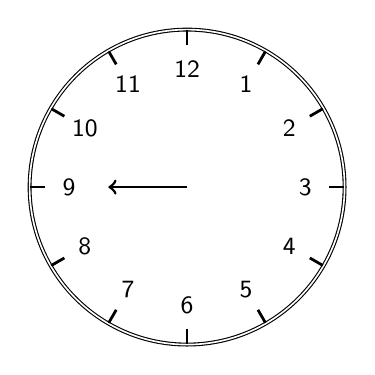
\begin{tikzpicture}[font=\small,x=6mm,y=6mm]
    \draw [double] (0,0) circle (2cm);
    \foreach \angle/ \label in{0/3, 30/2, 60/1, 90/12, 120/11, 150/10, 180/9,210/8, 240/7, 270/6, 300/5, 330/4}
    {
      \draw[line width=1pt] (\angle:1.8cm) -- (\angle:1.99cm);
      \draw (\angle:1.5cm) node{\textsf{\label}};
    }
      \draw[->,line width=1pt] (0,0) -- (180:1cm);
\end{tikzpicture}
 \caption{Esercizio~\ref{ese:E.8}.}\label{fig:E.10}
 \end{minipage}\hfil
 \begin{minipage}[t]{.45\textwidth}
 \centering% (c) 2012 Dimitrios Vrettos - d.vrettos@gmail.com
\begin{tikzpicture}[x=6mm,  y=6mm]
  \newcounter{num}
  \setcounter{num}{0}
  
  \draw[color=gray, step=6mm] (0,0) grid (8,10);
  \foreach \y in {9,8,...,0}{
    \foreach \x in {0,1,...,7}{
      \stepcounter{num}
      \ifnum \thenum<28
	\draw[xshift=3mm,yshift=3mm] (\x , \y ) node {\thenum};
      \fi
    }
  }
  
  \foreach \j in {10,9,8,...,0}
    \foreach \i in {0,1,...,8}
      \draw[] (\i , \j ) node[fill=white] {};
\end{tikzpicture}
 \caption{Esercizio~\ref{ese:E.9}.}\label{fig:E.11}
 \end{minipage}
\end{figure}


\subsubsection*{E.2 - Insiemi finiti e insiemi infiniti}

\begin{esercizio}
\label{ese:E.10}
Stabilisci la cardinalità dell'insieme~$V$ delle vocali della lingua italiana e dell'insieme~$D$ delle dita di una mano.

Completa l'insieme~$V$.

\`E possibile stabilire una corrispondenza biunivoca tra $V$ e $D$? Se sì, descrivila con una tabella.

Determina~$\insN_{5}$: \dotfill

Cosa si può dire sulla cardinalità di $V$, $D$ e $\insN_5$?
\end{esercizio}

\begin{esercizio}
\label{ese:E.11}
Negli insiemi ``infiniti'' non possiamo affermare che ``la parte è minore del tutto''.

Prolungate i lati obliqui
del trapezio~${ABCD}$ rappresentato nella figura~\ref{fig:E.12} fino a farli incontrare nel punto~$O$.
Le semirette di origine~$O$ e comprese tra~${OA}$ e~${OB}$, proiettano il segmento~${DC}$ sul segmento~${AB}$,
facendo così corrispondere ad un ogni punto di~${DC}$ un punto di~${AB}$.
Direste vera o falsa l'affermazione: <<i punti del segmento~${DC}$ sono tanti quanti quelli del segmento~${AB}$>>?

Seguite questi passaggi rispondendo ai quesiti:
\begin{enumeratea}
 \item quale punto di~$AB$ corrisponde a~$D$? e quale a~$C$?
 \item ogni punto di~${CD}$ trova un corrispondente punto in~${AB}$?
 \item di quale punto di~$DC$ è immagine il punto~$K$ di~${AB}$?
 \item ogni punto di~${AB}$ è immagine di un solo punto di~${CD}$?
 \item la proiezione costruita stabilisce una corrispondenza biunivoca tra~${CD}$ e~${AB}$?
 \item a quale conclusione vi ha condotto questo esercizio?
\end{enumeratea}
\end{esercizio}
\begin{figure}[htb]
  \centering% (c) 2012 Dimitrios Vrettos - d.vrettos@gmail.com
\begin{tikzpicture}[x=8mm, y=8mm]
\tkzDefPoint(0,0){A}
\tkzDefPoint(7,0){B}
\tkzDefPoint(4,3){C}
\tkzDefPoint(1,3){D}
\tkzDefPoint(4,0){K}

\tkzDrawPolygon(A, B, C, D)

\tkzLabelPoints[below](A, B, K)
\tkzLabelPoints[above](C, D)

\tkzSetUpPoint[fill=CornflowerBlue,size=6]
\tkzDrawPoints(A, B, C, D, K)

\end{tikzpicture}
 \caption{Esercizio~\ref{ese:E.11}.}\label{fig:E.12}
\end{figure}


\begin{esercizio}
\label{ese:E.12}
Gli insiemi~$A=\{x\mid x=2n^{2}-1$ con~$n\in \insN$ e~$0\le n<2\}$ e~$B=\{y\in \insZ\mid -1\le y\le 1\}$
si possono mettere in corrispondenza biunivoca?
\end{esercizio}

\begin{esercizio}
\label{ese:E.13}
Dato l'insieme~$K=\{$a, b, c, d$\}$, costruite l'insieme~$K\times K$.
Considerate il suo sottoinsieme~$H=\{(x;y)\in K\times K \mid x\text{ precede }y\text{ nell'ordine alfabetico}\}$.
\`E vero che tale insieme è equipotente all'insieme formato dalle facce di un cubo?
\end{esercizio}

\begin{esercizio}
\label{ese:E.14}
Attraverso la costruzione di un grafo sagittale, attribuite il valore di verità alla proposizione: ``il sottoinsieme~$T$ di
$\insN\times \insN$ formato dalle coppie i cui elementi danno come somma~$3$ è equipotente all'insieme~$F$ dei divisori di~$14$''.
\end{esercizio}

\begin{esercizio}
\label{ese:E.15}
\TabPositions{12cm}
Attribuite il valore di verità alle seguenti proposizioni:
 \begin{enumeratea}
\item un insieme infinito è sempre numerabile \tab\boxV\quad\boxF
\item un insieme infinito può essere equipotente a un suo sottoinsieme proprio \tab\boxV\quad\boxF
\item la cardinalità dell'insieme~$\insQ$ è maggiore di quella dell'insieme~$\insZ$ \tab\boxV\quad\boxF
\item due insiemi equipotenti sono infiniti \tab\boxV\quad\boxF
\end{enumeratea}
\end{esercizio}

\begin{esercizio}
\label{ese:E.16}

Considerando l'insieme~$P=\left\{2^{n}\text{ con }n\in \insN\right\}$ delle potenze di~$2$,
completa la tabella sottostante:
\begin{center}
 \begin{tabular}{cccccccccccc}
  \toprule
  $n$ & $0$ & $1$ & $2$ & $3$ & $4$ & $5$ & $6$ & $7$ & $8$ & $9$ & $\cdots$\\
  $2^n$ & $1$ & $2$ & & & & & & & & & $\cdots$ \\
  \bottomrule
 \end{tabular}
\end{center}

Qual è il valore di verità delle seguenti proposizioni?
\begin{enumeratea}
\TabPositions{8cm}
\item $P$ è un sottoinsieme di~$\insN$ \tab\boxV\quad\boxF
\item $0 \in P$ \tab\boxV\quad\boxF
\item $P$ è numerabile \tab\boxV\quad\boxF
\item nessun elemento di~$P$ è maggiore di~$\np{2065438}$\tab\boxV\quad\boxF
\end{enumeratea}

Quali considerazioni potete fare sull'infinità di~$P$?
\end{esercizio}

\subsubsection*{E.3 - Strutture algebriche}

\begin{esercizio}
\label{ese:E.17}
Rispondete ai seguenti quesiti:
\begin{enumeratea}
\item Cos'è una struttura algebrica?
\item Con quale scrittura la si rappresenta?
\item L'insieme $A=\{$1, 2, 3, 4, 5, 6, 7, 8, 9, 10$\}$ con l'operazione di addizione è una struttura algebrica? Perché?
\item L'insieme $P=\{x\in\insN\mid x$ è pari$\}$ con l'operazione di addizione è una struttura algebrica? Perché? E con l'operazione di moltiplicazione?
\item L'insieme $N_5=\{$0, 1, 2, 3, 4$\}$ con l'operazione di modulo (resto intero della divisione) è una struttura algebrica? Perché?
\end{enumeratea}
\end{esercizio}

\begin{esercizio}
\label{ese:E.18}
Dimostrare che $(\insQ$, $\star)$ con $a \star b=ab−a−b+2$ è un monoide.

\emph{Suggerimento:} L'operazione $\star$ è interna a $\insQ$? Gode della proprietà associativa? Qual è l'elemento neutro?
\end{esercizio}

\begin{esercizio}
\label{ese:E.19}
Dimostrare che $(\insZ$, $-$, $\cdot)$ è un anello commutativo con
identità e integro.
\end{esercizio}

\begin{esercizio}
\label{ese:E.20}
Dimostrare che $(\insR$, $+$, $\cdot)$ è un campo.
\end{esercizio}

\cleardoublepage
